%
% Vorlage
%
% Stefan Taber <stefan.taber@inso.tuwien.ac.at>
%
\documentclass[a4paper,11pt,german,public]{INSOexpose}
\usepackage{array,longtable}
\usepackage{setspace}
\usepackage{subfigure} 

\PassOptionsToPackage{hyphens}{url}
\usepackage{hyperref}
\usepackage{url}


\inputencoding{utf8} % linux, mac
% \inputencoding{latin1} % linux, mac

%
\title{\centering Evaluierung von REST Frameworks für Android im Kontext des Revex2020 Projekts\\}
% Bitte setzen falls der Titel zu lang ist
\shorttitle{Evaluierung von REST Frameworks}
\author{Elisabeth Pilz}
\matrikelnr{1225231}
\kennzahl{E 033 534}
\studium{Software \& Information Engineering}
\date{\today}
\dokumenttyp{Bachelorarbeit}
\assistent{}

% Bibliographie file
\bibliography{db}
%\ExecuteBibliographyOptions{sorting=none}
\begin{document}

\maketitle
\newgeometry{a4paper, top=3cm, left=3cm, bottom=3cm, right=3cm}
%=======================================================================
\section{Problemstellung}
%=======================================================================
%Allgemeine Problemstellung: Formulierung der konkreten Problemstellung in wenigen Sätzen. Welchem Themenbereich ist die Arbeit zuzuordnen?

Einer der größten Trends auf den Busniess Markt ist die Mobilisierung der Geschäftswelt, die sich in den verschiedensten Unternehmensstrategien widerspiegelt. Es gibt zahlreiche Innovatione, um unabhängig von Stackholdern, Zeit, Ort und Geräten auf Daten und Anwendungen zuzugreifen. Ein wesentlich Innovationsstrang ist dabei die Entwicklung von Business-Apps, um beispielsweise die Arbeitszeiten auf Geschäftsreisen effektiv ausnützen zu können. Dadurch hat die Bedeutung der Informations- und Kommunikationsindustrie (IKT) in den letzten Jahren in den Unternehmen stetig zugenommen\cite{smartMobileApps1}.
\\\\
Durch die immer stärkere Nachfrage nach mobilen Apps im Arbeitsalltag, ist es notwendig mobile Endgräte in bestehende Geschäftsprozesse der Unternehmen zu integrieren. Dabei soll es vermieden werden, eine komplett neue IT-Infrastruktur unter Beteiligung von mobilen Endgeräten zu schaffen. In vielen Unternehmen wird daher die IT-Anwendungslandschaft  an das Paradigma der Service-orientierten Architektur ausgerichtet. Ein wesentliche Vorteil dabei ist, dass wohl definierte Schnittstellen vorhanden sind und angebotene Dienste flexibel und plattformunabhängig genutzt werden können. Sollen nur mobile Anwendung in die existierende  IT-Anwendungslandschaft eingegliedert werden, bedeutet dies in der Service-orientierten Architektur, dass Web Services benötigt werden. In der Praxis werden Web Services entweder mit dem Kommunikationsprotokoll SOAP\footnote{Simple Object Access Protocol} oder REST\footnote{Representational State Transfer} umgesetzt \cite{smartMobileApps17}.
\\\\
Im  Revex2020 Projekt wird das Kommunikationsprotokoll REST verwendet, dadurch ist es maßgeblich ein geeignetes Framework auf Seiten der mobilen App zu finden, dass eine vollständige und korrekte Anbindung an das Webservice ermöglicht. Es existieren bereits zahlreiche Frameworks, die eine REST Implementierung unterstützen, diese unterscheiden sich aber stark in der Qualität. Auch bieten nicht alle diese Frameworks eine Unterstützung für Android an. Daher ist die Auswahl eines geeigneten Frameworks für eine erfolgreiche Implementierung  ausschlaggebend. 

%Das Projekt soll es Betreibern von Kleinwasserkraftwerken ermöglichen anhand von erfassten Daten aussagekräftige Bewertungen über den technischen Zustand von mechanischen, hydraulischen und elektrischen Kraftwerkskomponenten durchzuführen. So sollen z.B. Wartungskosten den Neuanschaffungskosten gegenübergestellt werden, um wirtschaftliche Entscheidungen zur Laufzeitverlängerung von Wasserkraftwerken treffen zu können.

%=======================================================================
\section{Zielsetzung/Motivation}
%=======================================================================
%Welches Ziel soll durch die Bachelorarbeit erreicht werden, was motiviert Sie zu dieser Arbeit? 

Die Thematik rund um die Evaluierung von REST-Frameworks für Android ist noch relativ neu, deswegen existieren noch nicht ausreichend genug Publikationen, um ein geeignetes Framework für das Projekt Revex2020 auszuwählen. Es gibt zwar einige Vergleiche von REST Frameworks, wie etwa die Fachstudie von Markus Fischer, Kalman Kepes und Alexander Wassiljew\cite{vergleich13}. In dieser Studie wird allerdings nicht darauf eingegangen, ob die Frameworks eine Implementierung clientseitig mit Android unterstützen. Dies ist aber eine essentielle Anforderung, da eine Business-App für Android entwickelt werden soll. 
\\\\
Der immer stärke wachsende Bereich von mobilen Anwendungen, macht das zu untersuchende Thema besonders interessant. Herkömmliche Software rückt immer weiter in den Hintergrund, Daten sollen sofort und überall abgerufen werden können. Mobile Endgeräte wie Smartphone und Tablets verändern daher die Geschäftswelt nachhaltig, Führungskräfte und Mitarbeiter erhalten jederzeit Zugang zu Unternehmensinformationen und -prozessen. Die Unternehmen der Zukunft sind daher mobil \cite{smartMobileApps7}.  
\\\\
Revex2020 ist ein Forschungsprojekt zur Revitalisierung von Wasserkraftwerken, das in Kooperation mit dem Institut für Energietechnik und Thermodynamik entwickelt wird \cite{projektbeschreibung:revex2020}. Ein Ziel dieses Projektes ist es, Mitarbeitern zukünftig zu ermöglichen, mithilfe von mobilen Endgeräten den Zustand einzelner Kraftwerkskomponenten vor Ort erfassen zu können. Es soll eine Android App entwickelt werden, die das bereits vorhandene Backend über das REST-Webservices nutzt um exemplarisch den Anwendungsfall abzubilden.
\\\\
Ziel dieser Bachelorarbeit ist die Evaluierung verschiedener REST-Frameworks für Android im Kontext des Revex2020 Projekts, um eine unkomplizierte Anbindung an das bereits vorhandene Backend zu ermöglichen. Dazu werden bestehende REST-Frameworks für Android getestet, indem diese in einem Anwendungsfall eingesetzt werden. Nach der Evaluierung dieser Frameworks soll eine Empfehlung abgegeben werden, welches sich am besten für das Revex2020 Projekt eignet.
\newpage
%=======================================================================
\section{Methodik}
%=======================================================================
%Werden theoretische, praktische oder empirische Analysen durchgeführt? Klare Darstellung der eingesetzten theoretischen und praktischen Methoden (Befragung, Recherche, Statistik, Rapid Prototyping, Objektorientierte Analyse, UML, Komponenten-basierte Entwicklung, Programmiersprachen etc.).

Die Evaluierung der Frameworks erfolgt anhand von Prototypen, indem die REST Frameworks verwendet werden. Es wurde im Vorfeld ein Anwendungsfall definiert, indem die einzelnen REST Frameworks  integriert werden. Dazu werden in einem Szenario verschiedene Prozess durchgespielt, wie Kraftwerk erstellen, löschen, bearbeiten und anzeigen. Als Vorlage dazu wird die bestehende Web-Applikation des Projektes verwendet.
\\\\
Die Qualität der einzelnen Frameworks soll anhand folgender Kriterien verglichen werden, welche an dem Kriterienkatalog der Fachstudie "Vergleich von Frameworks zur Implementierung von REST-basierten Anwendungen" \cite{vergleich13} angelehnt sind. Dieser Kriterienkatalog beschäftigt sich mit den Eigenschaften für die Evaluierung von REST Frameworks, vorallem aus serverseitigen Sicht. Dieser Katalog wurde deshalb gekürzt, sowie einzelne Punkte zusammengefasst und abgeändert um eine Evaluierung, im Kontext des Projektes Revex2020, durchführen zu können.
\\\\
\textbf{Allgemein:}
\begin{itemize}[label=$-$]
	\item Existiert eine aktive Community?
	\item Ist eine Dokumentation des Codes vorhanden? (Schnittstellenbeschreibung, JavaDoc)
	\item Unter welcher Lizenz steht das Projekt zur Verfügung=
	\item Gibt es Hilfestellung für Entwicklung? (Tutorial, Codebeispiele)
\end{itemize}

\textbf{Implementierung mit REST-Framework:}
\begin{itemize}[label=$-$]
	\item Wie lange wird benötigt um das Framework einzubinden?  (Zeitdauer)
	\item Welche HTTP-Verben werden unterstützt? (GET, POST, PUT, DELETE etc.)
	\item Gibt es Möglichkeiten den HTTP-Header zu verändern oder zu erweitern?
	\item Welche Medientypen werden unterstützt? (JSON, HTML, XML etc.)
	\item Wie erfolgt die Identifikation einzelner Ressourcen? (Aufruf der URL)
	\item Wird das HATEOAS Konzept unterstützt?
\end{itemize}

\textbf{Erweiterte Technische Fähigkeiten}
\begin{itemize}[label=$-$]
	\item Definiert das Framework eine eigene IDL\footnote{Schnittstellenbeschreibungssprachen}?
	\item Wie wird der Bereich Sicherheit gehandhabt?  (Authentifizierung, Verschlüsselung)
	\item Werden andere Protokolle außer HTTP noch unterstützt?
	\item Gibt es eine Möglichkeit für asynchronen Nachrichtenaustausch?
	\item Wird transaktionales Verhalten vom Framework unterstützt? (ACID-Eigenschaften)
\end{itemize}

%=======================================================================
\section{State of the Art}
%=======================================================================
%Welche Lösungen oder ähnlichen Projekte gibt es schon – Einbettung von Literaturzitaten (mind. 5); Fallbeispiele.
Um Rest Framework für die Evaluierung zu finden, wurde eine Technologie-Recherche durchgeführt. Dabei konnten folgende Projekte gefunden werden, welche eine REST Anbindung für Android unterstützen:
\begin{itemize}
	\item Resty (\href{http://beders.github.io/Resty/Resty/Overview.html}{http://beders.github.io/Resty/Resty/Overview.html})
	\item Retrofit (\href{http://square.github.io/retrofit/}{http://square.github.io/retrofit/})
	\item RESTlet (\href{http://restlet.com/}{http://restlet.com/})
	\item Spring for Android (\href{http://projects.spring.io/spring-android/}{http://projects.spring.io/spring-android/})
	\item CRest (\href{http://crest.codegist.org/index.html}{http://crest.codegist.org/index.html})
	\item RESTeasy Mobile (\href{http://resteasy.jboss.org/}{http://resteasy.jboss.org/})
	\item RESTDroid (\href{http://pcreations.fr/me/restdroid-resource-oriented-rest-client-for-android}{http://pcreations.fr/me/restdroid-resource-oriented-rest-client-for-android})
	\item Jersey (\href{https://jersey.java.net/}{https://jersey.java.net/})
\end{itemize}

\begin{figure}[!htbp]
	\centering	
	\subfigure[Diagramm: Github Stars]{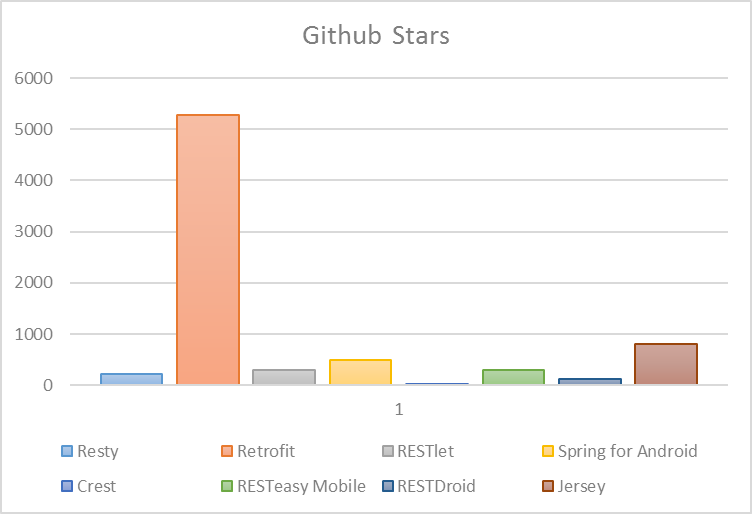
\includegraphics[width=0.8\textwidth]{imgs/github_stars.png}}
	\subfigure[Diagramm: Github Commits]{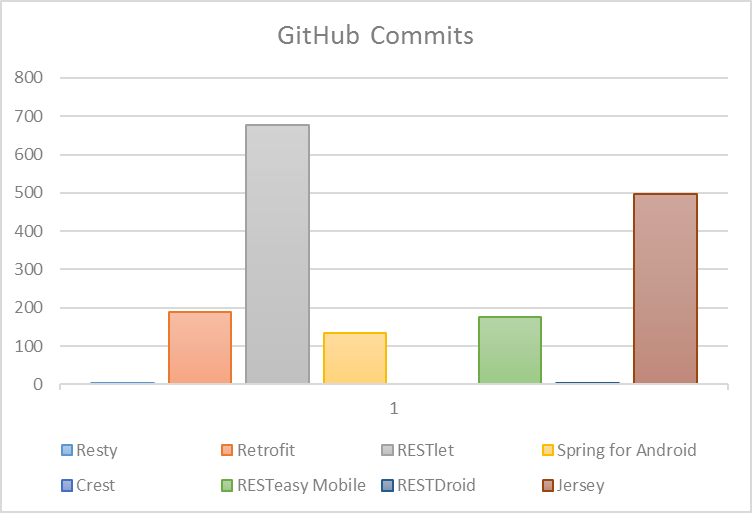
\includegraphics[width=0.8\textwidth]{imgs/github_commits.png}}
	\caption{Github Statistiken}	
	\label{figure:github}
\end{figure}

Es würde den Rahmen der Bachelorarbeit überschreiten, alle diese gefunden REST Frameworks zu evaluieren. Deswegen werden in einer Vorstudie die drei häufigsten und den Anforderungen entsprechenden Frameworks ausgewählt. Die Häufigkeit der Verwendung gibt oft eine gewisse Auskunft über die Qualität, da für diese Frameworks oft bessere Support zur Verfügung steht. Verschiedene Studien\cite{parnin2012crowd} beschäftigen sich damit wie Question and Answer (QA) Webseiten die Hilfestellung zu verschiedenen Frameworks verbessern. Diese wurden mithilfe von Github ermittelt, indem zu einem die Github Stars mit den Commits (seit dem 01.01.2014)  in den Repositories verglichen wurden, siehe Abbildung \ref{figure:github}. Es werden daher folgende REST-Frameworks evaluiert und miteinander verglichen:

\begin{itemize}
	\item Retrofit 
	\item Jersey
	\item Spring for Android
\end{itemize}

%=======================================================================
\section{Inhaltsverzeichnis}
%=======================================================================
Geplante Struktur der Arbeit: ca. 40 Seiten	
\begin{samepage}
  \begin{contentstructure}
    \item Einleitung	\estimatedpages{3 Seiten}
    \item State of the Art \estimatedpages{8 Seiten}
    \begin{contentstructure}
      \item Auswahl der Frameworks \estimatedpages{3 Seiten}
      \item Beschreibung der Frameworks \estimatedpages{5 Seiten}
    \end{contentstructure}
    \item Android \estimatedpages{7 Seiten}
    \begin{contentstructure}
      \item Aufbau \estimatedpages{2 Seiten}
      \item Prozess der App Implementierung \estimatedpages{5 Seiten}
    \end{contentstructure}
    \item Evaluierung der Frameworks \estimatedpages{9 Seiten}
    \begin{contentstructure}
      \item Framework 1	\estimatedpages{3 Seiten}
      \item Framework 2 \estimatedpages{3 Seiten}
      \item Framework 3 \estimatedpages{3 Seiten}
    \end{contentstructure}
    \item Ergebnis \estimatedpages{3 Seiten}
    \item Zusammenfassung \estimatedpages{2 Seiten}
  \end{contentstructure}
\end{samepage}

%=======================================================================
\section{Zeitplan}
%=======================================================================
Zeitplanung der geplanten Arbeit mit wichtigen Meilensteine.

\begin{spacing}{1.4}
\begin{longtable}{|p{.2 \linewidth}|p{.5 \linewidth}|}
	\hline
	\multicolumn{1}{|c|}{\textbf{Zeitraum}} & \textbf{Phase} \\ 
	\hline 
	Mitte Mai & Schreiben des Exposé \\ 
	\hline 
	Mitte Mai & Auswahl der Frameworks \\
	\hline 
	ab Mitte Mai & Erstellung der App mit ersten Framework \\
	\hline 
	Juni & Evaluierung der restlichen Frameworks \\
	\hline 
	Juni- Ende Juli & Schreiben des theoretischen Teils \\
	\hline
	\caption{Zeitplan}
	\label{tab:tabZeitplan}
\end{longtable}
\end{spacing}

\newpage
\nocite{dobjanschi:developing-android}
\nocite{tilko:rest}
\nocite{louis:android}
\nocite{stackOverflow:rest-client}
\nocite{burd:android}
% Bibliographie
\printbibliography

\end{document}
